\section{Current Operating-Model Evidence}

The cost and production layers inherited from Team 4 are purpose-built operating forecasts rather than generic statistical add-ons. They were first assembled in an earlier Barrick working paper that used a provisional Black--Scholes/GBM gold-price block. In the unified valuation only the operating method is retained and refreshed with Barrick's Q1--Q2 2026 mine statistics; the legacy gold-price simulation and illustrative EBITDA/valuation are excluded. This keeps the non-price inputs observable while ensuring that all valuation gold paths come from the current Team 8 engines.

\subsection{Cost-of-sales block}
The cost methodology stabilizes noisy mine-level CoS histories by extracting a common log-space market trend, forecasting that aggregate signal with the selected \textbf{ARIMA(3,1,0) with drift}, and reconstructing mine paths with volatility-scaled anchors. AIC and BIC select the aggregate specification at $-94.64$ and $-86.87$, respectively. Reported residual tests do not reject white noise or normality, while the 12-period hold-out produces a MAPE of $0.603\%$ and an RMSE approximately one third of the naive random-walk benchmark. These diagnostics support the model-selection step; they do not turn CoS into a jointly simulated state in the final valuation.

{\centering
  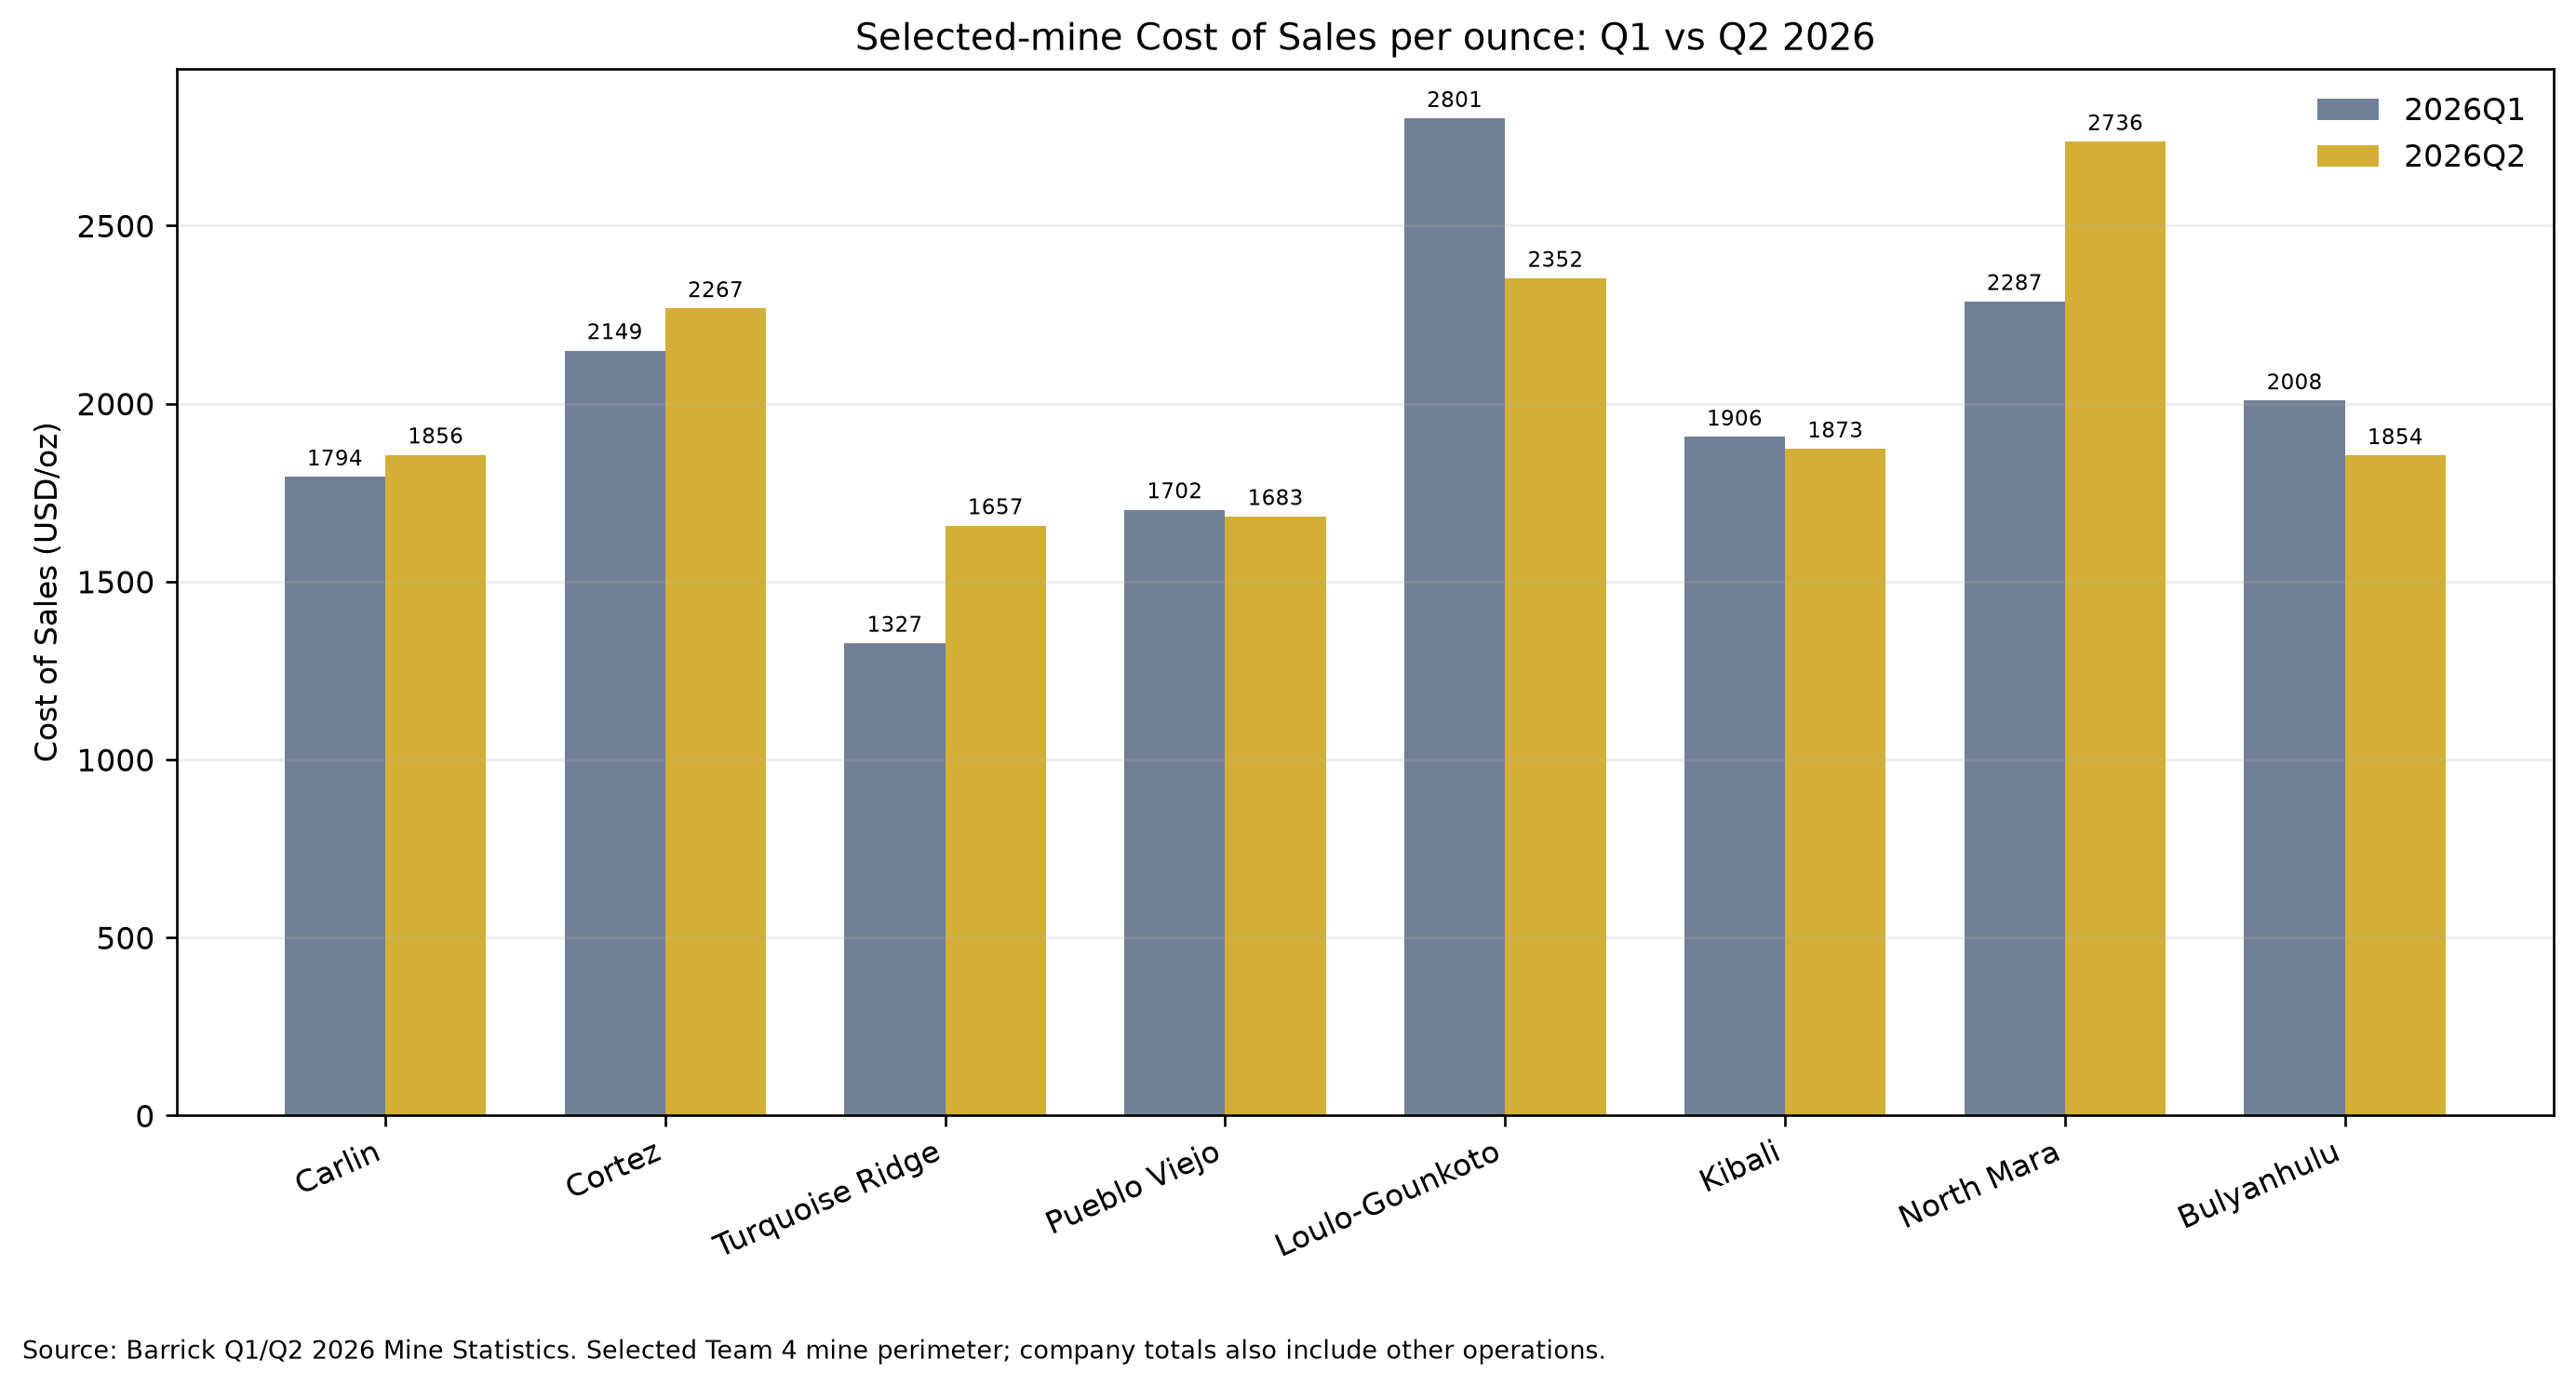
\includegraphics[width=0.95\columnwidth]{figures/team4_mine_cost_qoq.png}
  \captionof{figure}{Selected-mine Cost of Sales per ounce in Q1 and Q2 2026. Mine dispersion motivates preserving the Team 4 operating decomposition rather than replacing it with a single company-average cost.}
  \label{fig:team4_cost_qoq}
\par}

The refreshed actuals provide a transparent starting boundary for the operating forecast. From Q3 2026 onward, the unified experiment accepts the resulting deterministic 20-quarter cost vector rather than the fully stochastic CoS distributions explored in the source study. This design is intentional: simultaneous changes in gold, cost and production uncertainty would prevent clean attribution across the four price engines.

\subsection{Production block}
Production is modelled bottom-up rather than through a single total-output regression. Team 4 decomposes ounces into ore processed, average grade and recovery, using $SARIMA(1,0,1)(1,0,0)_4$ dynamics for ore, $SARIMA(1,0,0)(0,0,0)_4$ for grade and bounded stochastic simulation for recovery. The source does not report AIC/BIC selection for those production orders, so they are treated as admitted source specifications rather than re-selected models. Their physical recombination preserves mine heterogeneity and avoids the instability of a one-shot aggregate fit.

{\centering
  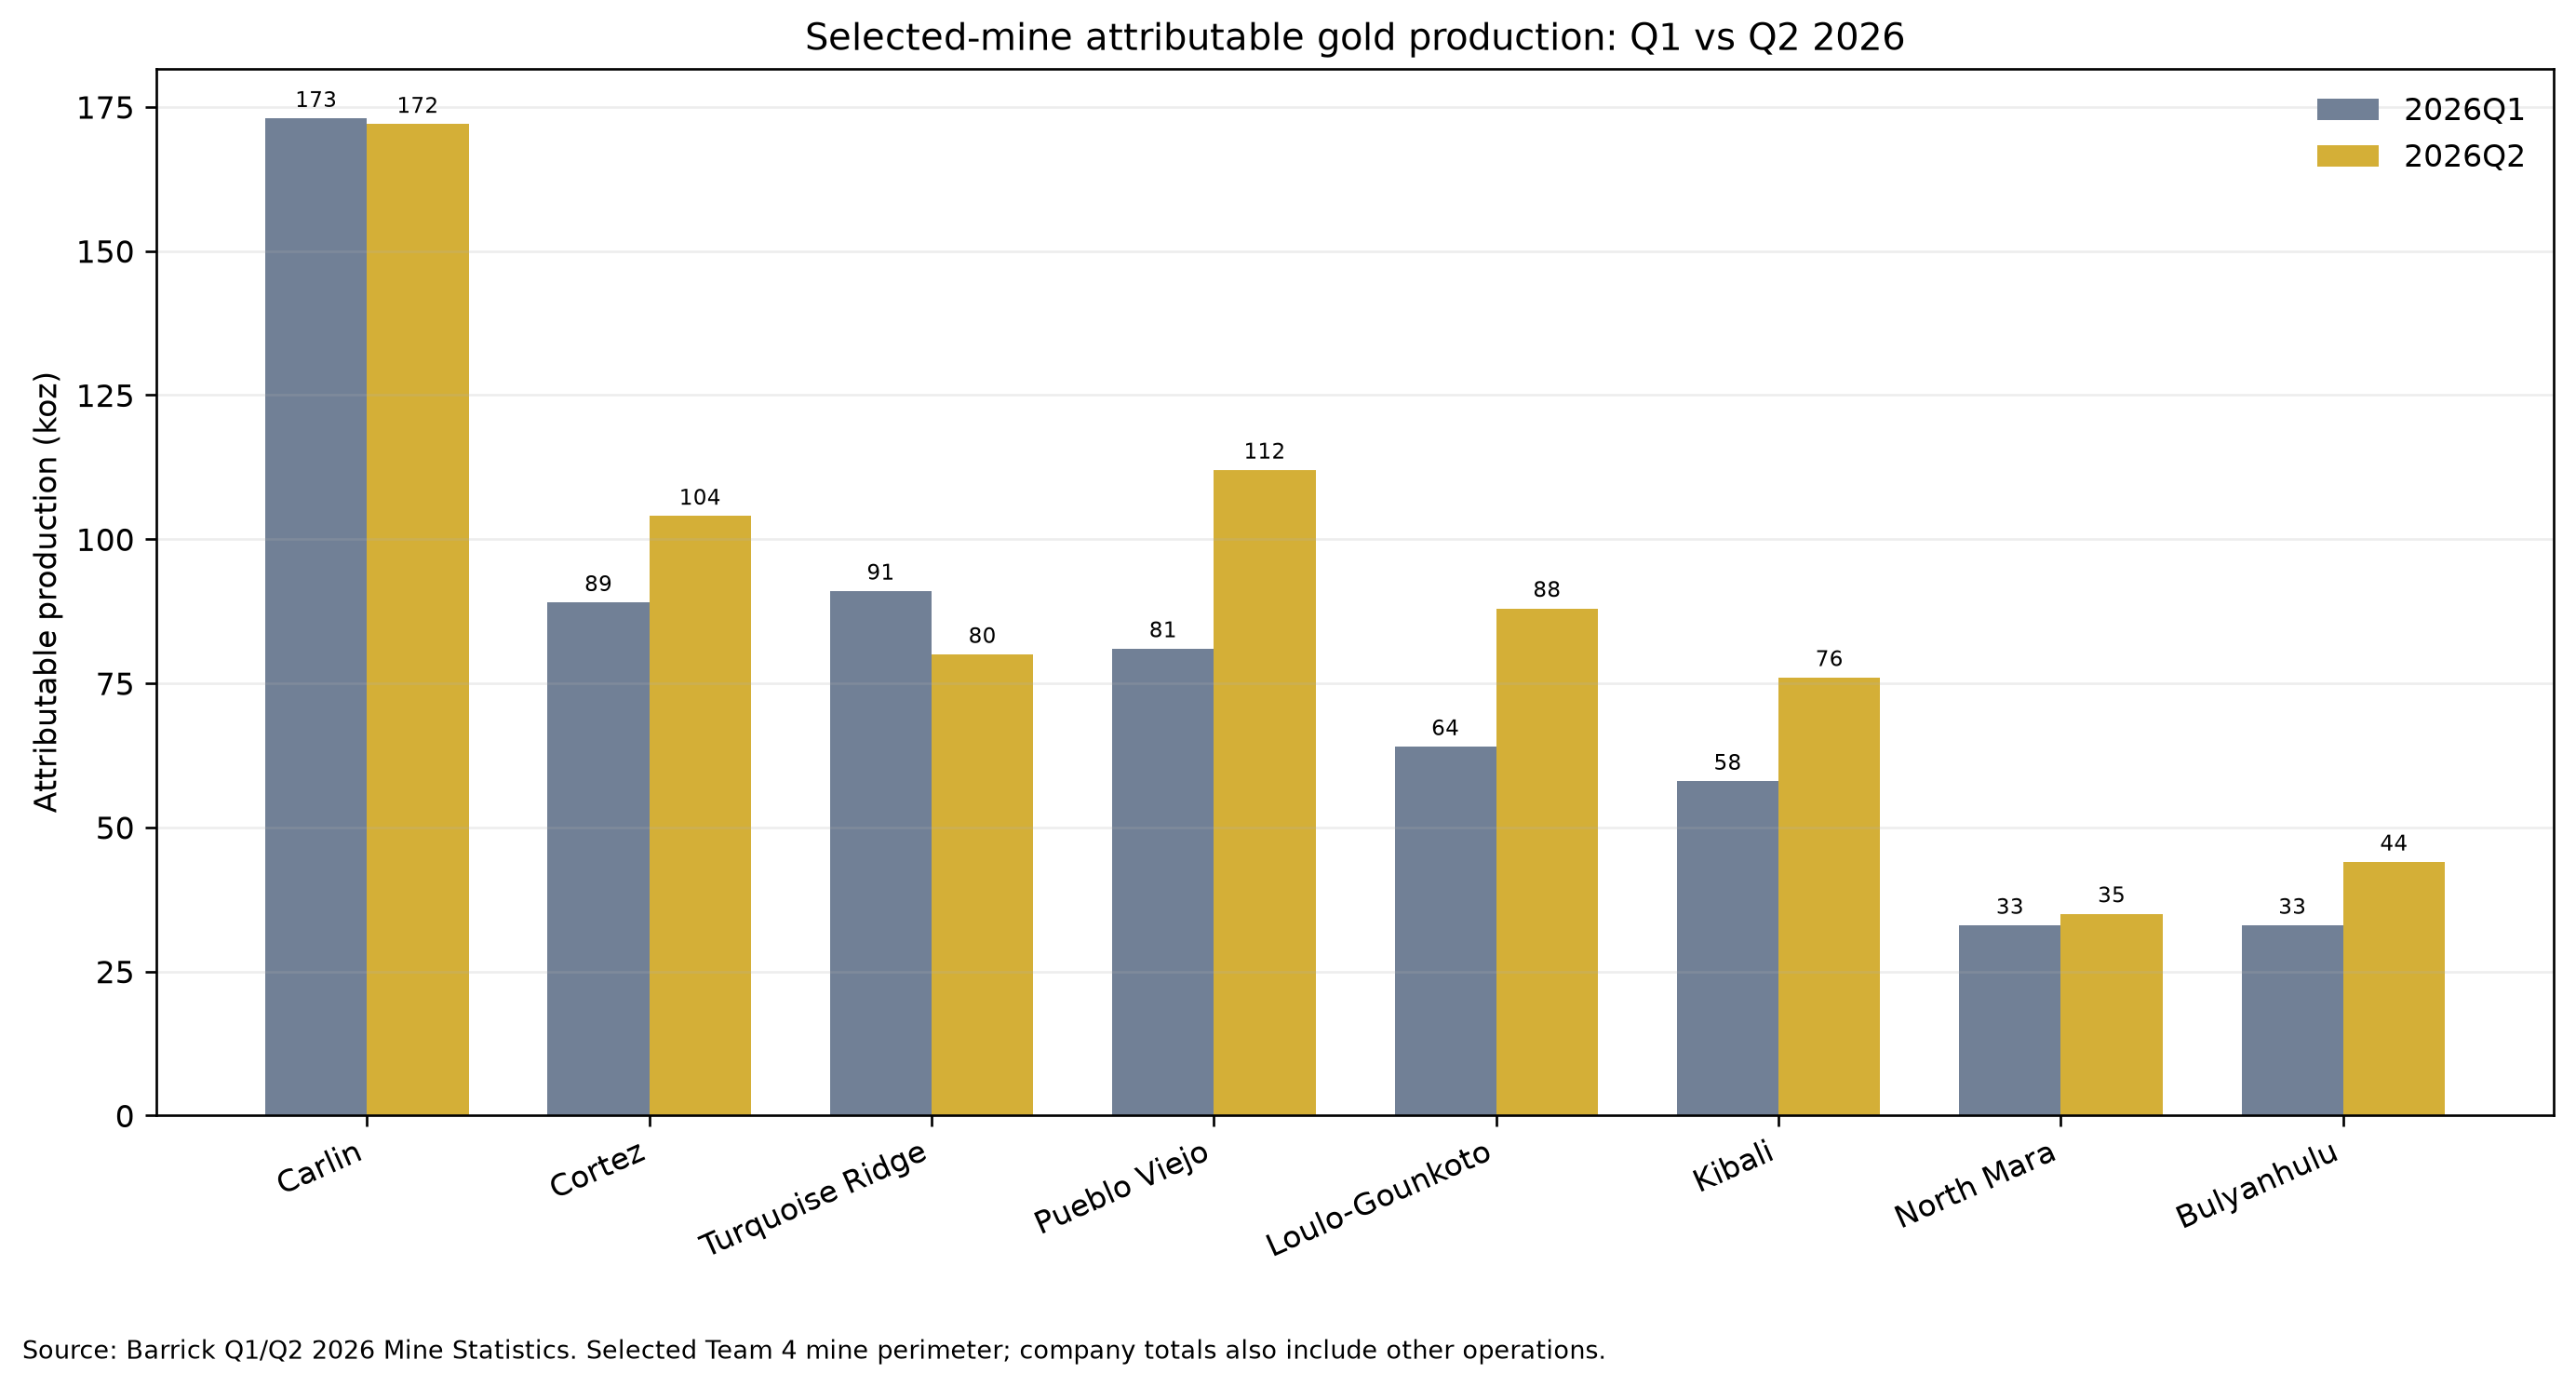
\includegraphics[width=0.95\columnwidth]{figures/team4_mine_production_qoq.png}
  \captionof{figure}{Selected-mine attributable gold production in Q1 and Q2 2026. The current actuals reveal heterogeneous changes that are hidden by a company-level total.}
  \label{fig:team4_production_qoq}
\par}

{\centering
  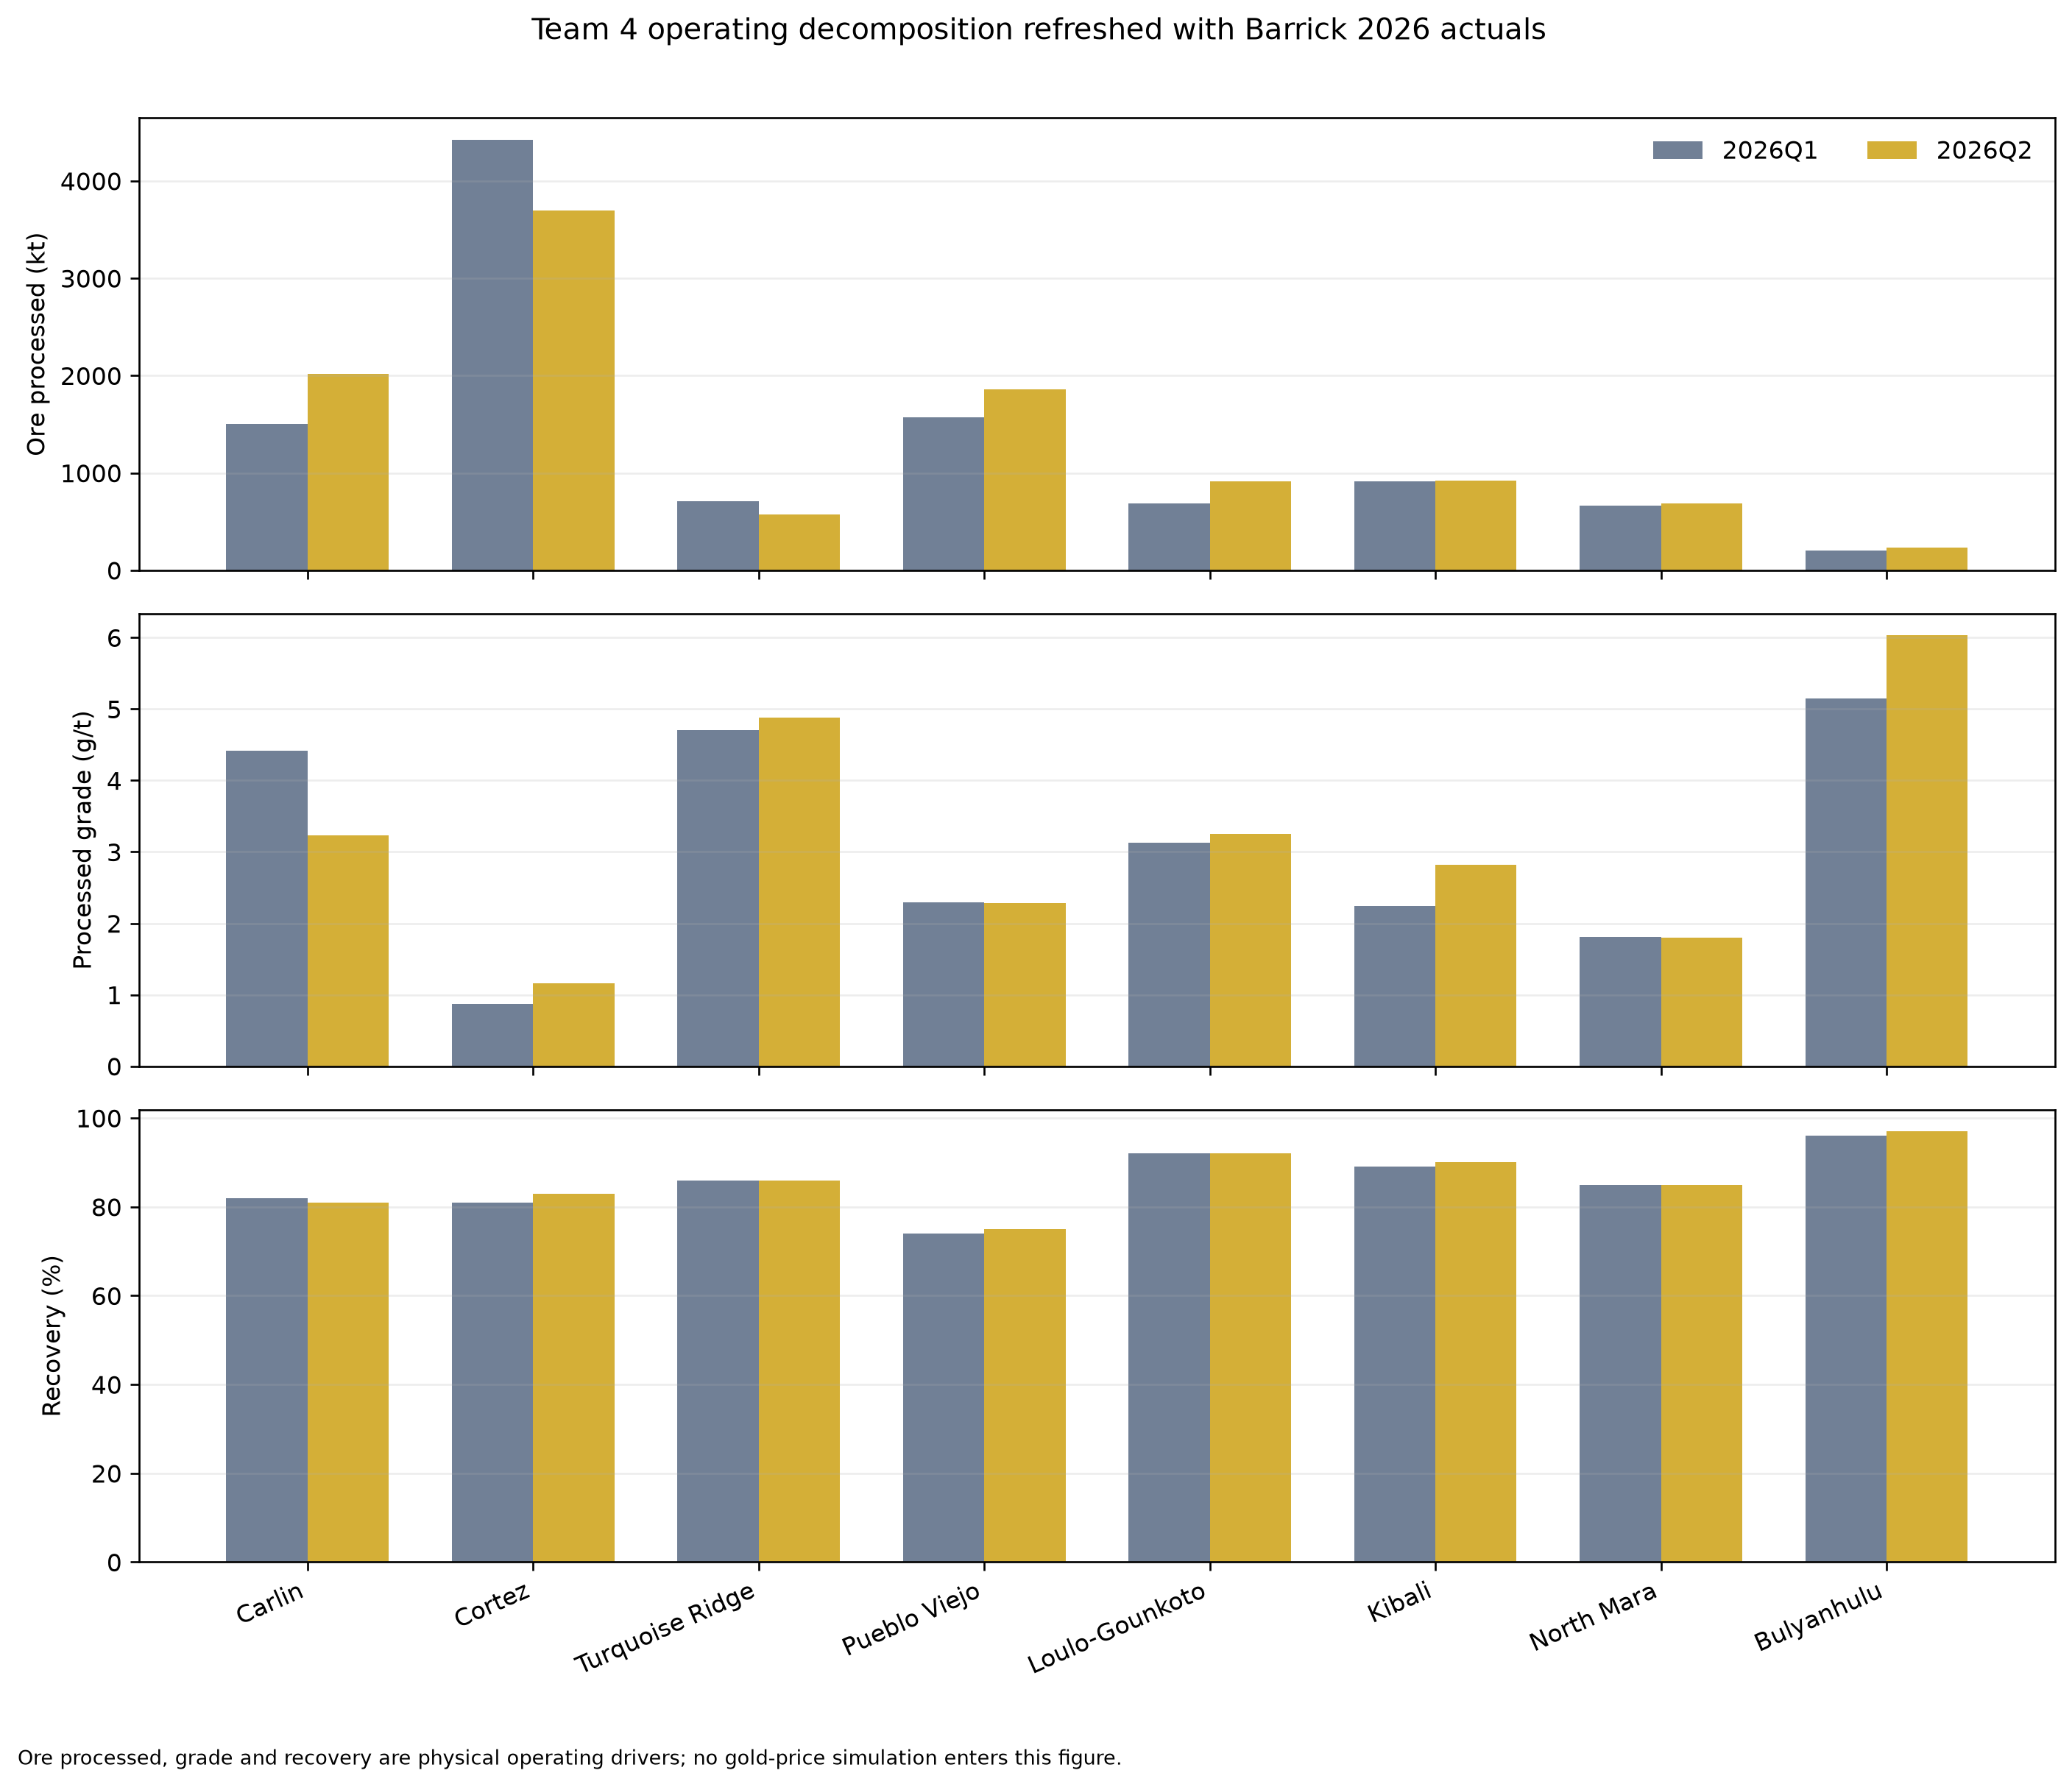
\includegraphics[width=0.95\columnwidth]{figures/team4_process_components_qoq.png}
  \captionof{figure}{Ore processed, grade and recovery updated with Barrick 2026 actuals. These are physical operating drivers; no commodity-price simulation enters the panel.}
  \label{fig:team4_process_qoq}
\par}

The original study also develops Goodman variance propagation and confidence bands for the production components. Those distributions remain useful evidence on operating-model uncertainty, but they are not propagated jointly in the four-engine corporate experiment: only the refreshed point vectors are passed downstream.

\subsection{Forecast handoff used by the valuation}
The final handoff keeps observed and modelled quantities distinct. Barrick's Q1--Q2 2026 actual production and CoS establish the current operating state; the Team 4 forecasts begin at Q3 2026 and extend through the common valuation horizon.

{\centering
  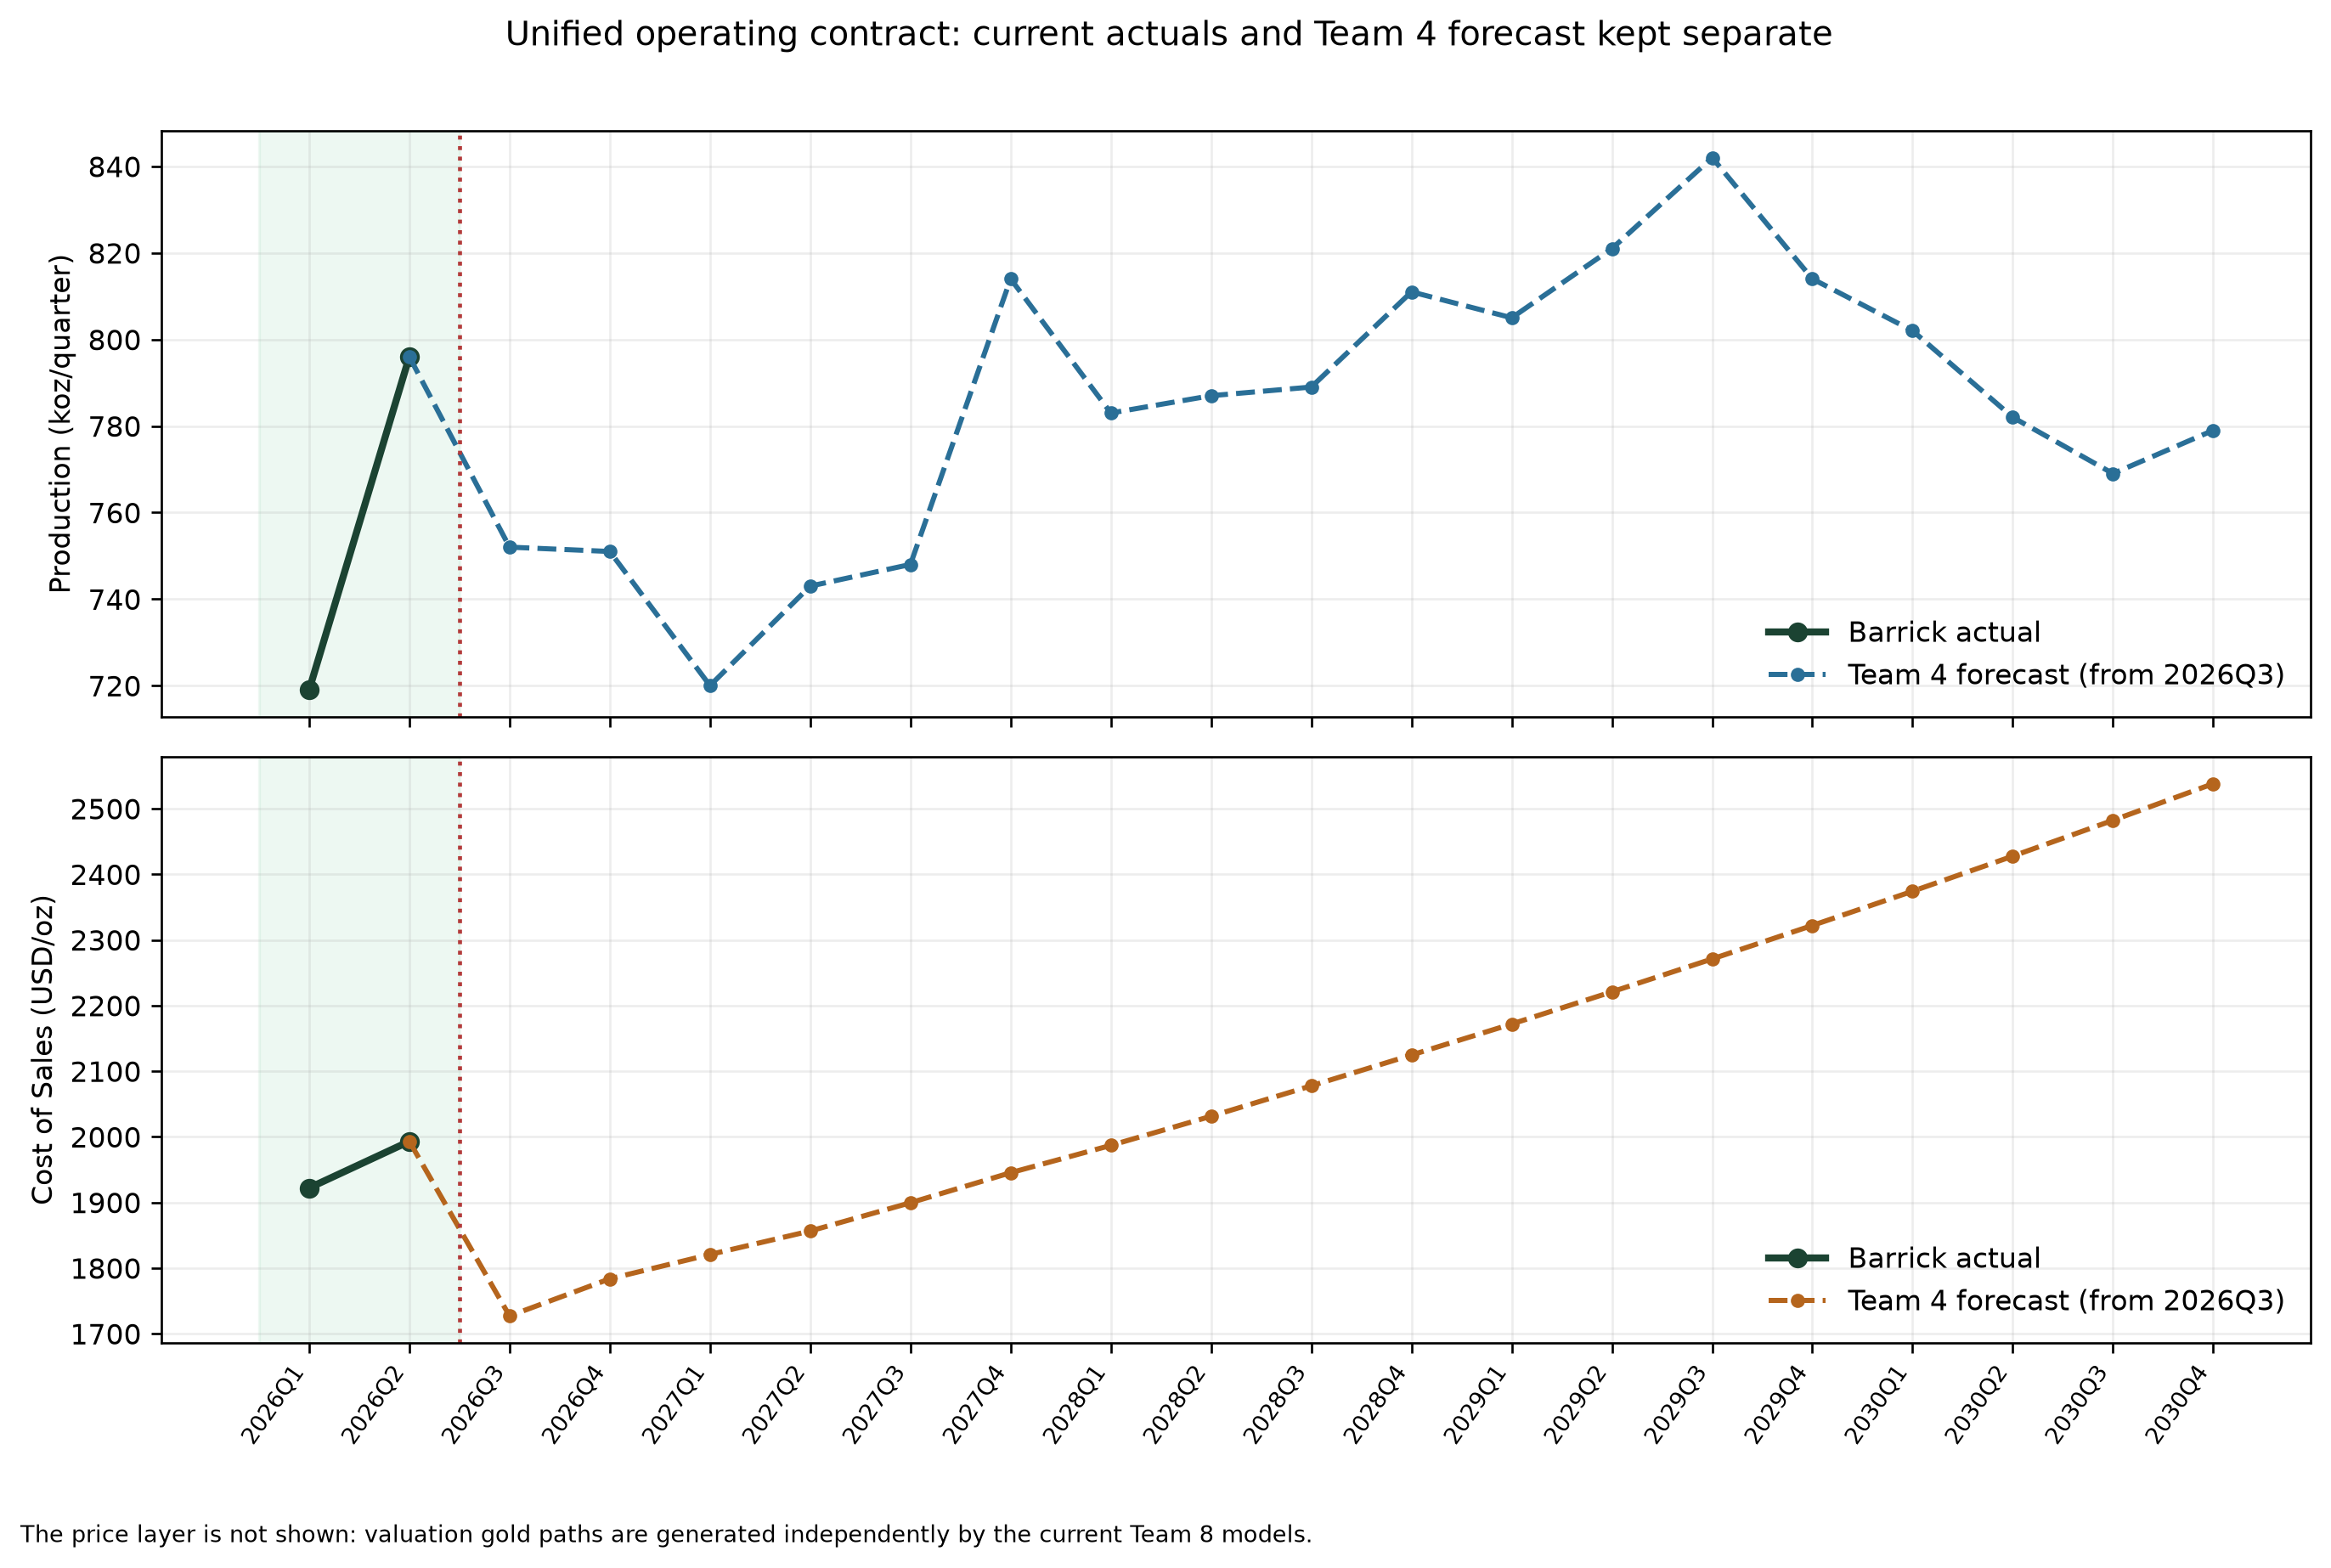
\includegraphics[width=0.95\columnwidth]{figures/team4_operating_contract.png}
  \captionof{figure}{Unified operating contract. Barrick Q1--Q2 2026 actuals are shown separately from the deterministic Team 4 production and CoS vectors used from Q3 2026 onward.}
  \label{fig:team4_contract}
\par}

\begin{methodbox}[Operating boundary]
The four valuation branches reuse the same refreshed production and cost vectors. Team 4's legacy gold-price and illustrative valuation outputs remain excluded, so differences in the final distributions can be attributed to the Team 8 gold-price process under a common Team 5 DCF contract.
\end{methodbox}
